\documentclass[12pt]{article}
\usepackage{fontspec}
\usepackage{xeCJK}
\setCJKmainfont[AutoFakeBold=2]{SimSun}
%\setCJKsansfont{SimHei}
\usepackage{amsmath, amssymb, amsthm}
\usepackage{geometry}
\usepackage{tikz}
\usepackage{fancyhdr}
%\setlength{\headheight}{15pt}
\usetikzlibrary{calc, intersections} % ABX 用於某些符號，若無可刪除
\usepackage{enumitem}
\usepackage{tkz-euclide}
\usepackage{subcaption}
\usepackage{indentfirst}
\usepackage{float}
\usepackage{chngcntr}
\counterwithin{figure}{section}
\usepackage[most]{tcolorbox}
\usepackage{etoolbox}
\usepackage{xcolor}
% 1. 定義一個新的開關，名字可以自訂（例如：showanswer）
\newtoggle{showanswer}

% 2. 設置開關狀態：true 為開啟（編譯），false 為關閉（不編譯）
\settoggle{showanswer}{true}

\newtcolorbox{mybox}[4][證明]{
  empty,
  breakable,                % 支援跨頁
  sharp corners,
  left=#2+#3,               % 為左側標籤預留空間 (縮進)
  right=0pt, top=0pt, bottom=0pt,
  colback=white,
  % --- 加入以下這行來調整段距 ---
  before upper={\setlength{\parskip}{0.5em plus 0.2em minus 0.1em}},
  after={\vspace{#4}},
  % ---------------------------
  overlay unbroken and first={ % 在第一頁/未斷頁時繪製標籤
    \node[
      anchor=north west,
      draw, 
      inner sep=0pt,
      minimum width=#2,
      minimum height=1.6em, 
      font=\bfseries\boldmath
    ] at (frame.north west) {#1};
  }
}

\geometry{left=1.5cm, right=1.5cm, top=2cm, bottom=2cm}
\counterwithout{figure}{subsection}
% 設定頁首頁尾
\pagestyle{fancy}
\fancyhf{}
\renewcommand{\headrulewidth}{2pt}
\renewcommand{\thefigure}{\thesection-\arabic{figure}} % 主圖編號 1-1
\renewcommand{\thesubfigure}{圖 \thesection-\arabic{figure}-\arabic{subfigure}} % 子圖變為 2-1-1
\captionsetup[figure]{labelformat=simple, labelsep=quad} 
\captionsetup[subfigure]{labelformat=simple, labelsep=quad} % 移除括號
\renewcommand{\figurename}{圖}
\lhead{廖汶鋒}
\chead{交比}
\rhead{澳門培道中學}
\fancyfoot[C]{\thepage} % Centered footer
%\fancyfoot[L]{2026年2月7日} % Left footer

%\title{四點共圓}
%\author{廖汶鋒}
%\date{2026年2月7日}
\linespread{1.3}

% 定段落首行縮進（兩個中文字）
\setlength{\parindent}{2em}
\setlength{\headheight}{15pt} % 避免頁首高度警告
\begin{document}
\thispagestyle{fancy}  % 讓首頁也顯示頁首
%\maketitle
\begin{center}
    \textbf{\Large{交比（Cross Ratio）}}
\end{center}

\indent 交比是射影幾何的一個重要概念，表面上是表示四個共線點的相對位置關係，實際是蘊含着射影幾何的不變性質。
在競賽幾何題中，交比是線段變換的重要工具，也是三點共線和三線共點的橋樑。

\begin{quotation}
    \centering
    \fbox{本內容為原創筆記，未經筆者允許，不得轉發。}
\end{quotation}
\section{線交比}
\begin{mybox}[定義]{4em}{1em}{0.5em}
    對於同一直線上的四個相異點$A$、$B$、$P$和$Q$，定義
    $$
        \left(A,B;P,Q\right)=\frac{\overrightarrow{AP}/\overrightarrow{PB}}{\overrightarrow{AQ}/\overrightarrow{QB}}
    $$
    稱$\left(A,B;P,Q\right)$為線段$AB$關於分點$P$和$Q$的\underline{線交比}；  
\end{mybox}
\begin{figure}[H]
    \centering
    \begin{subfigure}[b]{0.3\textwidth}
        \centering
        \begin{tikzpicture}[scale=0.8]
            \tkzDefPoints{-2/0/A, 2/0/B, 1/0/P, 3/0/Q}
            \tkzDrawPoints[fill=black](A,B,P,Q)
            \tkzDrawLine[black, thick, add = 0.1 and 0.1](A,Q)
            \tkzLabelPoints[above](A,B,P,Q)
        \end{tikzpicture}
        \caption{內分點及外分點}
        \label{fig:cr_in_out}
    \end{subfigure}
    \hfill
    \begin{subfigure}[b]{0.3\textwidth}
        \centering
        \begin{tikzpicture}[scale=0.8]
            \tkzDefPoints{-2/0/A, 2/0/B, 1/0/P, -0.5/0/Q}
            \tkzDrawPoints[fill=black](A,B,P,Q)
            \tkzDrawLine[black, thick, add = 0.1 and 0.1](A,B)
            \tkzLabelPoints[above](A,B,P,Q)
        \end{tikzpicture}
        \label{fig:cr_in_in}
        \caption{兩個內分點}
    \end{subfigure}
    \hfill
    \begin{subfigure}[b]{0.3\textwidth}
        \centering
        \begin{tikzpicture}[scale=0.8]
            \tkzDefPoints{-2/0/A, 1/0/B, -3/0/P, 2/0/Q}
            \tkzDrawPoints[fill=black](A,B,P,Q)
            \tkzDrawLine[black, thick, add = 0.1 and 0.1](P,Q)
            \tkzLabelPoints[above](A,B,P,Q)
        \end{tikzpicture}
        \label{fig:cr_out_out}
        \caption{兩個外分點}
    \end{subfigure}
    \caption{線交比的三種情況}
    \label{fig:cr_line}
\end{figure}
如果不採用有向比方式，有向交比亦可以寫成如下形式：
$$
    \left(A,B;P,Q\right)=s\left(AB;P,Q\right)\cdot\frac{AP/PB}{AQ/QB}
$$
其中$s\left(AB;P,Q\right)$是一個關於線段$AB$及其分點$P$及$Q$的正負號函數，表達式如下：
$$
    s\left(AB;P,Q\right)=\left\{\begin{matrix}
        +1,&P\text{、}Q\text{同為線段}AB\text{的內分點或外分點}\\
        -1,&\text{其餘情況}
    \end{matrix}\right.
$$
\section{圓交比}
\begin{mybox}[定義]{4em}{1em}{0.5em}
    對於同一圓$\Gamma$上的四個相異點$A$、$B$、$P$和$Q$，定義
    $$
        \left(A,B;P,Q\right)=s\left(AB;P,Q\right)\cdot\frac{AP/PB}{AQ/QB}
    $$
    稱$\left(A,B;P,Q\right)$為弧$AB$上的關於分點$P$和$Q$的\underline{圓交比}；
    \begin{figure}[H]
        \centering
        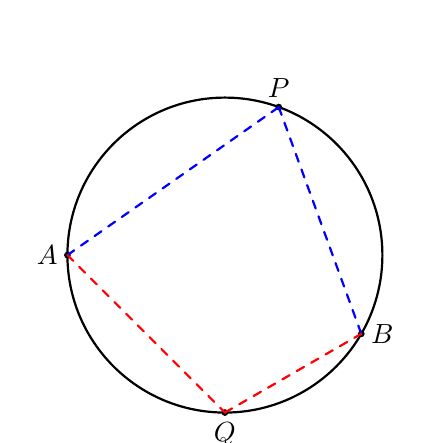
\begin{tikzpicture}[scale = 1.0]
            \tkzDefPoints{0/0/O, -2/0/A}
            \tkzDefPointBy[rotation= center O angle -110](A) \tkzGetPoint{P}
            \tkzDefPointBy[rotation= center O angle 90](A) \tkzGetPoint{Q}
            \tkzDefPointBy[rotation= center O angle 150](A) \tkzGetPoint{B}
            \tkzDrawPoints[black](A,B,P,Q)
            \tkzDrawCircle[black, thick](O,A)
            \tkzDrawSegments[blue, thick, dashed](A,P P,B)
            \tkzDrawSegments[red, thick, dashed](A,Q Q,B)
            \tkzLabelPoints[left](A)
            \tkzLabelPoints[above](P)
            \tkzLabelPoints[right](B)
            \tkzLabelPoints[below](Q)
        \end{tikzpicture}
        \label{fig:cr_circle}
        \caption{同一個圓上四點的交比}
    \end{figure}
    其中$s\left(AB;P,Q\right)$是一個關於弧$AB$及其分點$P$及$Q$的正負號函數，表達式如下：
    $$
        s\left(AB;P,Q\right)=\left\{\begin{matrix}
            +1,&P\text{、}Q\text{同為弧}AB\text{的內分點或外分點}\\
            -1,&\text{其餘情況}
        \end{matrix}\right.
    $$
    注意，在圓$\Gamma$上的弧$AB$有兩個，計算交比時，必須要選定同一條弧（優弧或劣弧）去討論、分析及計算。
\end{mybox}
可以留意到，圓交比與線交比的符號相同，在後續章節中將會介紹圓交比和線交比之間的聯繫。
\section{交比定理}
\begin{mybox}[定理1]{4.5em}{1em}{0.5em}
    在平面內任取一點$K$及四條通過$K$點的相異直線$\ell_1$、$\ell_2$、$\ell_3$和$\ell_4$。
    對於所有不通過$K$點的直線$\ell'$，使其與直線$\ell_1$、$\ell_2$、$\ell_3$和$\ell_4$相交於$A$、$B$、$P$和$Q$四點，
    則線分比滿足
    $$
        \left(A,B;P,Q\right)
        =\frac{\sin{\textcolor{red}{\measuredangle{\overrightarrow{AKP}}}}/\sin{\textcolor{red}{\measuredangle{\overrightarrow{PKB}}}}}
        {\sin{\textcolor{blue}{\measuredangle{\overrightarrow{AKQ}}}}/\sin{\textcolor{blue}{\measuredangle{\overrightarrow{QKB}}}}}
    $$
    \begin{figure}[H]
        \centering
        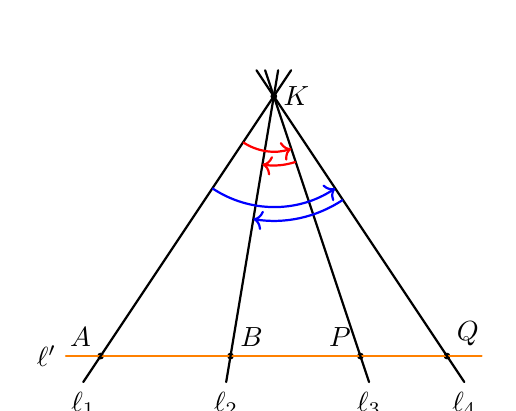
\begin{tikzpicture}[scale=1.1]
            \tkzDefPoints{-2/0/A, -0.5/0/B, 1/0/P, 2/0/Q, 0/3/K}         
            \tkzDrawPoints[fill=black](A,B,P,Q,K)
            \tkzDrawLine[orange, thick, add = 0.1 and 0.1](A,Q)
            \tkzDrawLines[black, thick, add = 0.1 and 0.1](K,A K,B K,P K,Q)
            \tkzLabelPoints[above right](B,Q)
            \tkzLabelPoints[above left](A,P)
            \tkzLabelPoint[right](K){$K$}
            \tkzLabelLine[below, pos=1.1](K,A){$\ell_1$}
            \tkzLabelLine[below, pos=1.1](K,B){$\ell_2$}
            \tkzLabelLine[below, pos=1.1](K,P){$\ell_3$}
            \tkzLabelLine[below, pos=1.1](K,Q){$\ell_4$}
            \tkzLabelLine[left, pos=-0.1](A,Q){$\ell'$}
            \tkzPicAngle[draw=red, thick, ->, angle radius = 20](A,K,P)
            \tkzPicAngle[draw=red, thick, <-, angle radius = 25](B,K,P)
            \tkzPicAngle[draw=blue, thick, ->, angle radius = 40](A,K,Q)
            \tkzPicAngle[draw=blue, thick, <-, angle radius = 45](B,K,Q)
        \end{tikzpicture}  
        \caption{線交比定理}
        \label{fig:cr_bundle_Line}
    \end{figure}
\end{mybox}
\begin{mybox}{4.5em}{1em}{0.5em}
    利用有向分角定理可知
    \begin{equation*}
        \frac{\overrightarrow{AP}}{\overrightarrow{PB}}
        =\frac{\sin{\measuredangle{\overrightarrow{AKP}}}}{\sin{\measuredangle{\overrightarrow{PKB}}}}
        \cdot\frac{KA}{KB},\hspace{2em} \frac{\overrightarrow{AQ}}{\overrightarrow{QB}}
        =\frac{\sin{\measuredangle{\overrightarrow{AKQ}}}}{\sin{\measuredangle{\overrightarrow{QKB}}}}
        \cdot\frac{KA}{KB}
    \end{equation*}
    上述兩式相除可得
    \begin{equation*}
        \left(A,B;P,Q\right)=\frac{\sin{\measuredangle{\overrightarrow{AKP}}}/\sin{\measuredangle{\overrightarrow{PKB}}}}
        {\sin{\measuredangle{\overrightarrow{AKQ}}}/\sin{\measuredangle{\overrightarrow{QKB}}}}
    \end{equation*}
\end{mybox}
\begin{mybox}[定理2]{4.5em}{1em}{0.5em}
    在平面內任取一點$K$及通過$K$點的圓$\Gamma$。在圓$\Gamma$上任取四點$A$、$B$、$P$和$Q$，
    則圓分比滿足
    $$
        \left(A,B;P,Q\right)
        =\frac{\sin{\textcolor{red}{\measuredangle{\overrightarrow{AKP}}}}/\sin{\textcolor{red}{\measuredangle{\overrightarrow{PKB}}}}}
        {\sin{\textcolor{blue}{\measuredangle{\overrightarrow{AKQ}}}}/\sin{\textcolor{blue}{\measuredangle{\overrightarrow{QKB}}}}}
    $$
    \begin{figure}[H]
        \centering
        \begin{subfigure}[p]{0.4\textwidth}
            \centering
            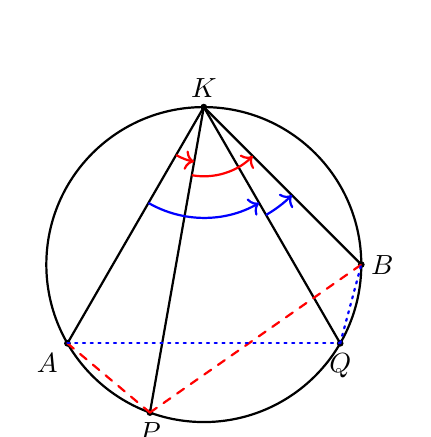
\begin{tikzpicture}[scale=2]
                \tkzDefPoints{0/0/O, 0/1/K}
                \tkzDefPointBy[rotation=center O angle 120](K)  \tkzGetPoint{A}
                \tkzDefPointBy[rotation=center O angle 160](K)  \tkzGetPoint{P}
                \tkzDefPointBy[rotation=center O angle 240](K)  \tkzGetPoint{Q}
                \tkzDefPointBy[rotation=center O angle 270](K)  \tkzGetPoint{B}
                \tkzDrawPoints[fill=black](A,B,P,Q,K)
                \tkzDrawCircle[black, thick](O,K)
                \tkzDrawSegments[black, thick](K,A K,B K,P K,Q)
                \tkzDrawSegments[red, thick, dashed](A,P P,B)
                \tkzDrawSegments[blue, thick, dotted](A,Q Q,B)
                \tkzLabelPoints[below](P,Q)
                \tkzLabelPoint[below left](A){$A$}
                \tkzLabelPoint[right](B){$B$}
                \tkzLabelPoint[above](K){$K$}
                \tkzPicAngle[draw=red, thick, ->, angle radius = 20](A,K,P)
                \tkzPicAngle[draw=red, thick, ->, angle radius = 25](P,K,B)
                \tkzPicAngle[draw=blue, thick, ->, angle radius = 40](A,K,Q)
                \tkzPicAngle[draw=blue, thick, ->, angle radius = 45](Q,K,B)
            \end{tikzpicture}  
            \caption{情況一}
            \label{fig:cr_bundle_Circle_1}
        \end{subfigure}
        \hfill
        \begin{subfigure}[p]{0.4\textwidth}
            \centering
            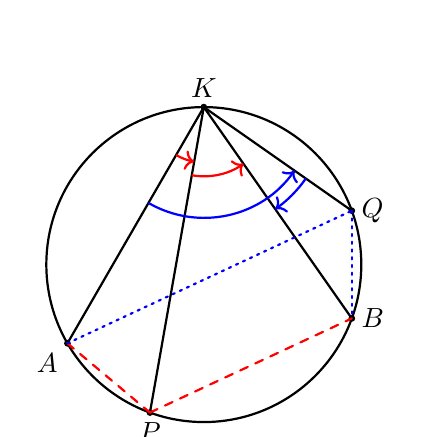
\begin{tikzpicture}[scale=2]
                \tkzDefPoints{0/0/O, 0/1/K}
                \tkzDefPointBy[rotation=center O angle 120](K)  \tkzGetPoint{A}
                \tkzDefPointBy[rotation=center O angle 160](K)  \tkzGetPoint{P}
                \tkzDefPointBy[rotation=center O angle 290](K)  \tkzGetPoint{Q}
                \tkzDefPointBy[rotation=center O angle 250](K)  \tkzGetPoint{B}
                \tkzDrawPoints[fill=black](A,B,P,Q,K)
                \tkzDrawCircle[black, thick](O,K)
                \tkzDrawSegments[black, thick](K,A K,B K,P K,Q)
                \tkzDrawSegments[red, thick, dashed](A,P P,B)
                \tkzDrawSegments[blue, thick, dotted](A,Q Q,B)
                \tkzLabelPoints[below](P)
                \tkzLabelPoint[below left](A){$A$}
                \tkzLabelPoints[right](B,Q)
                \tkzLabelPoint[above](K){$K$}
                \tkzPicAngle[draw=red, thick, ->, angle radius = 20](A,K,P)
                \tkzPicAngle[draw=red, thick, ->, angle radius = 25](P,K,B)
                \tkzPicAngle[draw=blue, thick, ->, angle radius = 40](A,K,Q)
                \tkzPicAngle[draw=blue, thick, <-, angle radius = 45](B,K,Q)
            \end{tikzpicture}  
            \caption{情況二}
            \label{fig:cr_bundle_Circle_2}
        \end{subfigure}
        \caption{圓交比的兩種情況}
        \label{fig:cr_bundle_Circle}
    \end{figure}
\end{mybox}
\begin{mybox}{4.5em}{1em}{0.5em}
    由正弦定理可知
    $$
        \left|\frac{\sin{\measuredangle{\overrightarrow{AKP}}}}{\sin{\measuredangle{\overrightarrow{PKB}}}}\right|=\frac{\sin{\angle{AKP}}}{\sin{\angle{PKB}}}=\frac{AP}{PB}
    $$
    $$
        \left|\frac{\sin{\measuredangle{\overrightarrow{AKQ}}}}{\sin{\measuredangle{\overrightarrow{QKB}}}}\right|=\frac{\sin{\angle{AKQ}}}{\sin{\angle{QKB}}}=\frac{AQ}{QB}
    $$
    所以有
    $$
        \left|\frac{\sin{\measuredangle{\overrightarrow{AKP}}}/\sin{\measuredangle{\overrightarrow{PKB}}}}{\sin{\measuredangle{\overrightarrow{AKQ}}}/\sin{\measuredangle{\overrightarrow{QKB}}}}\right|=\frac{AP/PB}{AQ/QB}
    $$
    接下來只需要討論待求證的等式之右式的正負號即可：
    \begin{itemize}
        \item $\sin{\measuredangle{\overrightarrow{AKP}}}/\sin{\measuredangle{\overrightarrow{PKB}}}>0$當且僅當$P$點是$\angle{AKB}$所對圓弧$AB$的內分點。
        \item $\sin{\measuredangle{\overrightarrow{AKQ}}}/\sin{\measuredangle{\overrightarrow{QKB}}}>0$當且僅當$Q$點是$\angle{AKB}$所對圓弧$AB$的內分點。
    \end{itemize}
    結合實數的符號運算原則可知
    $$
        \frac{\sin{\measuredangle{\overrightarrow{AKP}}}/\sin{\measuredangle{\overrightarrow{PKB}}}}{\sin{\measuredangle{\overrightarrow{AKQ}}}/\sin{\measuredangle{\overrightarrow{QKB}}}}>0\Leftrightarrow P\text{、}Q\text{同為}\angle{AKB}\text{所對圓弧}AB\text{內分點或外分點}
    $$
    即
    $$
        sgn\left(\frac{\sin{\measuredangle{\overrightarrow{AKP}}}/\sin{\measuredangle{\overrightarrow{PKB}}}}{\sin{\measuredangle{\overrightarrow{AKQ}}}/\sin{\measuredangle{\overrightarrow{QKB}}}}\right)=s\left(AB,P,Q\right)
    $$
    其中$sgn:\mathbb{R}\setminus\left\{1\right\}\rightarrow\left\{-1,1\right\}$是符號函數
    $$
        sgn(x)=\left\{\begin{matrix}
            +1,&x>0\\
            -1,&x<0
        \end{matrix}\right.=\frac{x}{\left|x\right|}
    $$
    因此可得
    \begin{align*}
        \frac{\sin{\measuredangle{\overrightarrow{AKP}}}/\sin{\measuredangle{\overrightarrow{PKB}}}}{\sin{\measuredangle{\overrightarrow{AKQ}}}/\sin{\measuredangle{\overrightarrow{QKB}}}}&=
        sgn\left(\frac{\sin{\measuredangle{\overrightarrow{AKP}}}/\sin{\measuredangle{\overrightarrow{PKB}}}}{\sin{\measuredangle{\overrightarrow{AKQ}}}/\sin{\measuredangle{\overrightarrow{QKB}}}}\right)\cdot\left|\frac{\sin{\measuredangle{\overrightarrow{AKP}}}/\sin{\measuredangle{\overrightarrow{PKB}}}}{\sin{\measuredangle{\overrightarrow{AKQ}}}/\sin{\measuredangle{\overrightarrow{QKB}}}}\right|\\
        &=s\left(AB,P,Q\right)\cdot\frac{AP/PB}{AQ/QB}\\
        &=\left(A,B;P,Q\right)
    \end{align*}
\end{mybox}
上述的四條共點直線（$KA$、$KB$、$KP$、$KQ$）稱為「共點四線束」。觀察定理1、定理2、圖\ref{fig:cr_bundle_Line}、圖\ref{fig:cr_bundle_Circle}，
直線$\ell$或圓$\Gamma$與共點四線束相交而生成的四個交點，其交比與\fbox{直線$\ell$或圓$\Gamma$的相對位置\textbf{無關}}，
只與\fbox{共點四線束的夾角（有向角）\textbf{有關}}。
\section{交比的性質}
以下性質的名稱為筆者自創，讀者於數學競賽時，可直接使用交比的性質。
本章節都默認以下前提：\underline{$A$、$B$、$P$和$Q$四點共線於$\ell$或共圓於$\Gamma$。}
\begin{mybox}[性質1]{4.5em}{1em}{0.5em}
    端點-分點對交換性：$\left(A,B;P,Q\right)=\left(P,Q;A,B\right)$；
\end{mybox}
\begin{mybox}{4.5em}{1em}{0.5em}
    按照以下兩個原則選取$K$點：
    \begin{itemize}
        \item 若$A$、$B$、$P$和$Q$四點共線於$\ell$，則在直線$\ell$外任取一點為$K$點；
        \item 若$A$、$B$、$P$和$Q$四點共圓於$\Gamma$，則在圓$\Gamma$上任取一點為$K$點，且$K\notin\left\{A,B,P,Q\right\}$；
    \end{itemize}
    基於以上兩個原則，我們都可以利用交比定理：
    \begin{align*}
        \left(A,B;P,Q\right)&=\frac{\sin{\measuredangle{\overrightarrow{AKP}}}/\sin{\measuredangle{\overrightarrow{PKB}}}}{\sin{\measuredangle{\overrightarrow{AKQ}}}/\sin{\measuredangle{\overrightarrow{QKB}}}}=\frac{\sin{\measuredangle{\overrightarrow{AKP}}}\cdot\sin{\measuredangle{\overrightarrow{QKB}}}}{\sin{\measuredangle{\overrightarrow{AKQ}}}\cdot\sin{\measuredangle{\overrightarrow{PKB}}}}\\
        &=\frac{\sin{\measuredangle{\overrightarrow{PKA}}}\cdot\sin{\measuredangle{\overrightarrow{BKQ}}}}{\sin{\measuredangle{\overrightarrow{AKQ}}}\cdot\sin{\measuredangle{\overrightarrow{PKB}}}}=\frac{\sin{\measuredangle{\overrightarrow{PKA}}}/\sin{\measuredangle{\overrightarrow{AKQ}}}}{\sin{\measuredangle{\overrightarrow{PKB}}}/\sin{\measuredangle{\overrightarrow{BKQ}}}}\\
        &=\left(P,Q;A,B\right)
    \end{align*}
\end{mybox}
\begin{mybox}[性質2]{4.5em}{1em}{0.5em}
    端點-分點倒數性：$\left(A,B;P,Q\right)=\left(A,B;Q,P\right)^{-1}=\left(B,A;P,Q\right)^{-1}$；
\end{mybox}
\begin{mybox}{4.5em}{1em}{0.5em}
    同樣按照上一個證明的原則去選取$K$點，利用交比定理可得
    \begin{align*}
        \left(A,B;P,Q\right)&=\frac{\sin{\measuredangle{\overrightarrow{AKP}}}/\sin{\measuredangle{\overrightarrow{PKB}}}}{\sin{\measuredangle{\overrightarrow{AKQ}}}/\sin{\measuredangle{\overrightarrow{QKB}}}}\\
        &=\left(\frac{\sin{\measuredangle{\overrightarrow{AKQ}}}/\sin{\measuredangle{\overrightarrow{QKB}}}}{\sin{\measuredangle{\overrightarrow{AKP}}}/\sin{\measuredangle{\overrightarrow{PKB}}}}\right)^{-1}=\left(A,B;Q,P\right)^{-1}
    \end{align*}
    再結合性質1可得
    $$
        \left(A,B;P,Q\right)=\left(P,Q;A,B\right)=\left(P,Q;B,A\right)^{-1}=\left(B,A;P,Q\right)^{-1}
    $$
\end{mybox}
\begin{mybox}[性質3]{4.5em}{1em}{0.5em}
    線-線射影不變性：若$A$、$B$、$P$和$Q$四點共線於$\ell$，任取直線$\ell$外的一點$K$
    以及一條不通過$K$點的直線$\ell'$，使其與直線$KA$、$KB$、$KP$和$KQ$分別相交於$A'$、$B'$、$P'$和$Q'$，
    均有以下關係成立：
    $$
        \left(A,B;P,Q\right)=\left(A',B';P',Q'\right)
    $$
    \begin{figure}[H]
        \centering
        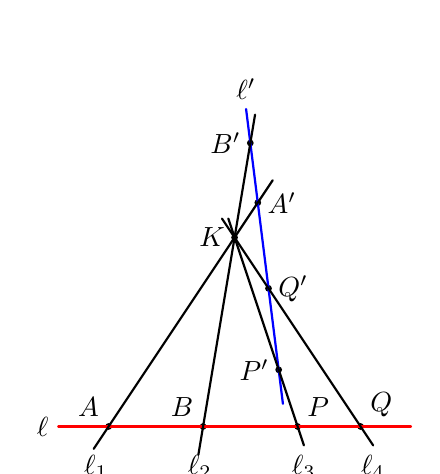
\begin{tikzpicture}[scale=0.8]
            \tkzDefPoints{-2/0/A, -0.5/0/B, 1/0/P, 2/0/Q, 0/3/K}         
            \tkzDefPointOnLine[pos = 0.7](K,P) \tkzGetPoint{P'}
            \tkzDefPointOnLine[pos = -0.5](K,B) \tkzGetPoint{B'}
            \tkzInterLL(K,A)(P',B') \tkzGetPoint{A'}
            \tkzInterLL(K,Q)(P',B') \tkzGetPoint{Q'}
            \tkzDrawPoints[fill=black](A,B,P,Q,K,A',B',P',Q')
            \tkzDrawLine[red, thick, add = 0.2 and 0.2](A,Q)
            \tkzDrawLine[blue, thick, add = 0.15 and 0.15](P',B')
            \tkzDrawLines[black, thick, add = 0.1 and 0.1](A,A' B,B' K,P K,Q)
            \tkzLabelLine[below, pos=1.1](K,A){$\ell_1$}
            \tkzLabelLine[below, pos=1.1](K,B){$\ell_2$}
            \tkzLabelLine[below, pos=1.1](K,P){$\ell_3$}
            \tkzLabelLine[below, pos=1.1](K,Q){$\ell_4$}
            \tkzLabelLine[left, pos=-0.2](A,Q){$\ell$}
            \tkzLabelLine[above, pos=-0.15](B',P'){$\ell'$}
            \tkzLabelPoints[above left](A,B)
            \tkzLabelPoints[above right](P,Q)
            \tkzLabelPoints[left](K)
            \tkzLabelPoints[left](B',P')
            \tkzLabelPoints[right](A',Q')
        \end{tikzpicture}
        \caption{線-線射影不變性}
        \label{fig:cr_ll_0}
    \end{figure}
\end{mybox}
\begin{mybox}{4.5em}{1em}{0.5em}
    根據定理1可知，兩個交點點列的線交比分別是
    \begin{equation*}
        \left(A,B;P,Q\right)=\frac{\sin{\measuredangle{\overrightarrow{AKP}}}/\sin{\measuredangle{\overrightarrow{PKB}}}}
        {\sin{\measuredangle{\overrightarrow{AKQ}}}/\sin{\measuredangle{\overrightarrow{QKB}}}},\hspace{2em}
        \left(A',B';P',Q'\right)=\frac{\sin{\measuredangle{\overrightarrow{A'KP'}}}/\sin{\measuredangle{\overrightarrow{P'KB'}}}}
        {\sin{\measuredangle{\overrightarrow{A'KQ'}}}/\sin{\measuredangle{\overrightarrow{Q'KB'}}}}
    \end{equation*}
    對於任意線段$XY$及其上的分點$Z$，其中$Z\notin\left\{X,Y\right\}$，定義一個函數$g\left(XY;Z\right)$：
    $$
        g\left(XY;Z\right)=\begin{cases}
            1,&\text{若$Z$是$XY$的內分點}\\
            0,&\text{若$Z$是$XY$的外分點}
        \end{cases}
    $$
    觀察$\measuredangle{\overrightarrow{A'KP'}}$可知
    $$
        \measuredangle{\overrightarrow{A'KP'}}=
        \measuredangle{\overrightarrow{A'KA}}+\measuredangle{\overrightarrow{AKP}}+\measuredangle{\overrightarrow{PKP'}}
        =\measuredangle{\overrightarrow{AKP}}+g\left(AA';K\right)\pi+g\left(PP';K\right)\pi
    $$
    所以有
    $$
        \sin{\measuredangle{\overrightarrow{A'KP'}}}=(-1)^{g\left(AA';K\right)+g\left(PP';K\right)}\sin{\measuredangle{\overrightarrow{AKP}}}
    $$
    同理可得
    \begin{align*}
        \sin{\measuredangle{\overrightarrow{P'KB'}}}&=(-1)^{g\left(PP';K\right)+g\left(BB';K\right)}\sin{\measuredangle{\overrightarrow{PKB}}}\\
        \sin{\measuredangle{\overrightarrow{A'KQ'}}}&=(-1)^{g\left(AA';K\right)+g\left(QQ';K\right)}\sin{\measuredangle{\overrightarrow{AKQ}}}\\
        \sin{\measuredangle{\overrightarrow{Q'KB'}}}&=(-1)^{g\left(QQ';K\right)+g\left(BB';K\right)}\sin{\measuredangle{\overrightarrow{QKB}}}
    \end{align*}
    因此有
    \begin{align*}
        \frac{\sin{\measuredangle{\overrightarrow{A'KP'}}}/\sin{\measuredangle{\overrightarrow{P'KB'}}}}
        {\sin{\measuredangle{\overrightarrow{A'KQ'}}}/\sin{\measuredangle{\overrightarrow{Q'KB'}}}}
        &=\frac{(-1)^{g\left(AA';K\right)-g\left(PP';K\right)-g\left(PP';K\right)+g\left(BB';K\right)}}{(-1)^{g\left(AA';K\right)-g\left(QQ';K\right)-g\left(QQ';K\right)+g\left(BB';K\right)}}
        \frac{\sin{\measuredangle{\overrightarrow{AKP}}}/\sin{\measuredangle{\overrightarrow{AKQ}}}}{\sin{\measuredangle{\overrightarrow{PKB}}}/\sin{\measuredangle{\overrightarrow{QKB}}}}\\
        &=\frac{\sin{\measuredangle{\overrightarrow{AKP}}}/\sin{\measuredangle{\overrightarrow{AKQ}}}}{\sin{\measuredangle{\overrightarrow{PKB}}}/\sin{\measuredangle{\overrightarrow{QKB}}}}
    \end{align*}
    即有
    $$
        \left(A,B;P,Q\right)=\left(A',B';P',Q'\right)
    $$
\end{mybox}
\begin{mybox}[性質3的其他情況]{9.5em}{1em}{0.5em}
    關於定理3，點列$\left(A,B,P,Q\right)$與點列$\left(A',B',P',Q'\right)$還有其他不同的分佈情況，任何一種情況都滿足線-線射影不變性。
    以下列舉四種不同的情況，讀者可以自行驗證其正確性。
\end{mybox}
\begin{figure}[H]
    \centering
    \begin{subfigure}[b]{0.4\textwidth}
        \centering
        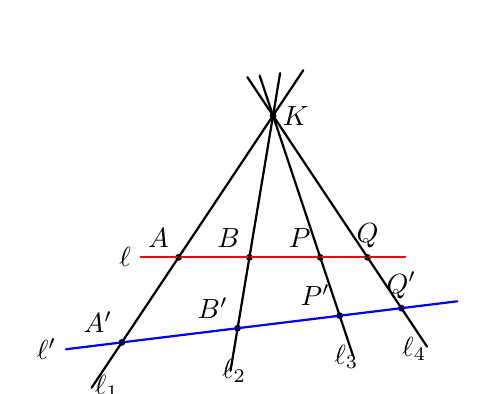
\begin{tikzpicture}[scale=0.6]
            \tkzDefPoints{-2/0/A, -0.5/0/B, 1/0/P, 2/0/Q, 0/3/K}         
            \tkzDefPointOnLine[pos = 1.6](K,A) \tkzGetPoint{A'}
            \tkzDefPointOnLine[pos = 1.5](K,B) \tkzGetPoint{B'}
            \tkzInterLL(K,P)(A',B') \tkzGetPoint{P'}
            \tkzInterLL(K,Q)(A',B') \tkzGetPoint{Q'}
            \tkzDrawPoints[fill=black](A,B,P,Q,K,A',B',P',Q')
            \tkzDrawLine[red, thick, add = 0.2 and 0.2](A,Q)
            \tkzDrawLine[blue, thick, add = 0.2 and 0.2](A',Q')
            \tkzDrawLines[black, thick, add = 0.2 and 0.2](K,A' K,B' K,P' K,Q')
            \tkzLabelLine[below, pos=1.1](K,A'){$\ell_1$}
            \tkzLabelLine[below, pos=1.1](K,B'){$\ell_2$}
            \tkzLabelLine[below, pos=1.1](K,P'){$\ell_3$}
            \tkzLabelLine[below, pos=1.1](K,Q'){$\ell_4$}
            \tkzLabelLine[left, pos=-0.2](A,Q){$\ell$}
            \tkzLabelLine[left, pos=-0.2](A',Q'){$\ell'$}
            \tkzLabelPoints[above left](A,B,P)
            \tkzLabelPoints[above](Q)
            \tkzLabelPoints[right](K)
            \tkzLabelPoints[above left](A',B',P')
            \tkzLabelPoints[above](Q')
        \end{tikzpicture}
        \caption{情況一}
        \label{fig:cr_ll_1}
    \end{subfigure}
    \hfill
    \begin{subfigure}[b]{0.4\textwidth}
        \centering
        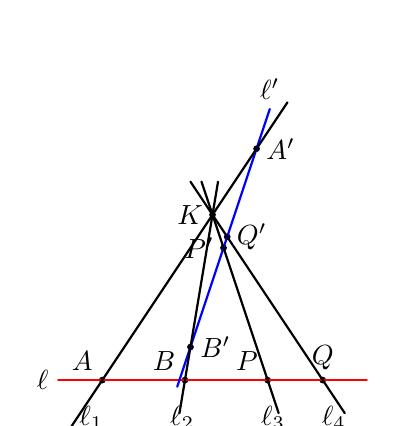
\begin{tikzpicture}[scale=0.7]
            \tkzDefPoints{-2/0/A, -0.5/0/B, 1/0/P, 2/0/Q, 0/3/K}         
            \tkzDefPointOnLine[pos = -0.4](K,A) \tkzGetPoint{A'}
            \tkzDefPointOnLine[pos = 0.8](K,B) \tkzGetPoint{B'}
            \tkzInterLL(K,P)(A',B') \tkzGetPoint{P'}
            \tkzInterLL(K,Q)(A',B') \tkzGetPoint{Q'}
            \tkzDrawPoints[fill=black](A,B,P,Q,K,A',B',P',Q')
            \tkzDrawLine[red, thick, add = 0.2 and 0.2](A,Q)
            \tkzDrawLine[blue, thick, add = 0.2 and 0.2](A',B')
            \tkzDrawLines[black, thick, add = 0.2 and 0.2](A,A' K,B K,P K,Q)
            \tkzLabelLine[below, pos=1.1](K,A){$\ell_1$}
            \tkzLabelLine[below, pos=1.1](K,B){$\ell_2$}
            \tkzLabelLine[below, pos=1.1](K,P){$\ell_3$}
            \tkzLabelLine[below, pos=1.1](K,Q){$\ell_4$}
            \tkzLabelLine[left, pos=-0.2](A,Q){$\ell$}
            \tkzLabelLine[above, pos=-0.2](A',B'){$\ell'$}
            \tkzLabelPoints[above left](A,B,P)
            \tkzLabelPoints[above](Q)
            \tkzLabelPoints[left](K)
            \tkzLabelPoints[left](P')
            \tkzLabelPoints[right](A',B',Q')
        \end{tikzpicture}
        \caption{情況二}
        \label{fig:cr_ll_2}
    \end{subfigure}
    \vspace{1em}
    \begin{subfigure}[b]{0.4\textwidth}
        \centering
        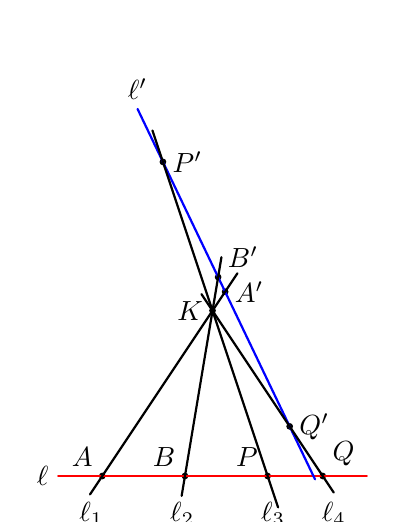
\begin{tikzpicture}[scale=0.7]
            \tkzDefPoints{-2/0/A, -0.5/0/B, 1/0/P, 2/0/Q, 0/3/K}         
            \tkzDefPointOnLine[pos = -0.9](K,P) \tkzGetPoint{P'}
            \tkzDefPointOnLine[pos = 0.7](K,Q) \tkzGetPoint{Q'}
            \tkzInterLL(K,A)(P',Q') \tkzGetPoint{A'}
            \tkzInterLL(K,B)(P',Q') \tkzGetPoint{B'}
            \tkzDrawPoints[fill=black](A,B,P,Q,K,A',B',P',Q')
            \tkzDrawLine[red, thick, add = 0.2 and 0.2](A,Q)
            \tkzDrawLine[blue, thick, add = 0.2 and 0.2](P',Q')
            \tkzDrawLines[black, thick, add = 0.1 and 0.1](A,A' B,B' P,P' K,Q)
            \tkzLabelLine[below, pos=1.1](K,A){$\ell_1$}
            \tkzLabelLine[below, pos=1.1](K,B){$\ell_2$}
            \tkzLabelLine[below, pos=1.1](K,P){$\ell_3$}
            \tkzLabelLine[below, pos=1.1](K,Q){$\ell_4$}
            \tkzLabelLine[left, pos=-0.2](A,Q){$\ell$}
            \tkzLabelLine[above, pos=-0.2](P',Q'){$\ell'$}
            \tkzLabelPoints[above left](A,B,P)
            \tkzLabelPoints[above right](Q)
            \tkzLabelPoints[left](K)
            \tkzLabelPoints[above right](B')
            \tkzLabelPoints[right](A',P',Q')
        \end{tikzpicture}
        \caption{情況三}
        \label{fig:cr_ll_3}
    \end{subfigure}
    \hfill
    \begin{subfigure}[b]{0.4\textwidth}
        \centering
        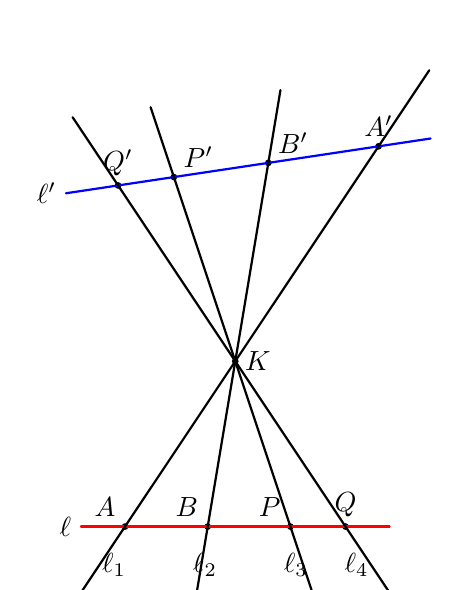
\begin{tikzpicture}[scale=0.7]
            \tkzDefPoints{-2/0/A, -0.5/0/B, 1/0/P, 2/0/Q, 0/3/K}         
            \tkzDefPointOnLine[pos = -1.3](K,A) \tkzGetPoint{A'}
            \tkzDefPointOnLine[pos = -1.2](K,B) \tkzGetPoint{B'}
            \tkzInterLL(K,P)(A',B') \tkzGetPoint{P'}
            \tkzInterLL(K,Q)(A',B') \tkzGetPoint{Q'}
            \tkzDrawPoints[fill=black](A,B,P,Q,K,A',B',P',Q')
            \tkzDrawLine[red, thick, add = 0.2 and 0.2](A,Q)
            \tkzDrawLine[blue, thick, add = 0.2 and 0.2](A',Q')
            \tkzDrawLines[black, thick, add = 0.2 and 0.2](A,A' B,B' P,P' Q,Q')
            \tkzLabelLine[below, pos=1.1](K,A){$\ell_1$}
            \tkzLabelLine[below, pos=1.1](K,B){$\ell_2$}
            \tkzLabelLine[below, pos=1.1](K,P){$\ell_3$}
            \tkzLabelLine[below, pos=1.1](K,Q){$\ell_4$}
            \tkzLabelLine[left, pos=-0.2](A,Q){$\ell$}
            \tkzLabelLine[left, pos=-0.2](Q',A'){$\ell'$}
            \tkzLabelPoints[above left](A,B,P)
            \tkzLabelPoints[above](Q)
            \tkzLabelPoints[right](K)
            \tkzLabelPoints[above](A',Q')
            \tkzLabelPoints[above right](B',P')
        \end{tikzpicture}
        \caption{情況四}
        \label{fig:cr_ll_4}
    \end{subfigure}         
\end{figure}
\begin{mybox}[性質4]{4.5em}{1em}{0.5em}
線-圓射影不變性：若$A$、$B$、$P$和$Q$四點共線於$\ell$，任取直線$\ell$外的一點$K$
以及一個通過$K$點的圓$\Sigma$，使其與直線$KA$、$KB$、$KP$和$KQ$分別相交於$A'$、$B'$、$P'$和$Q'$，
均有以下關係成立：
$$
    \left(A',B';P',Q'\right)=\left(A,B;P,Q\right)
$$
\begin{figure}[H]
    \centering
    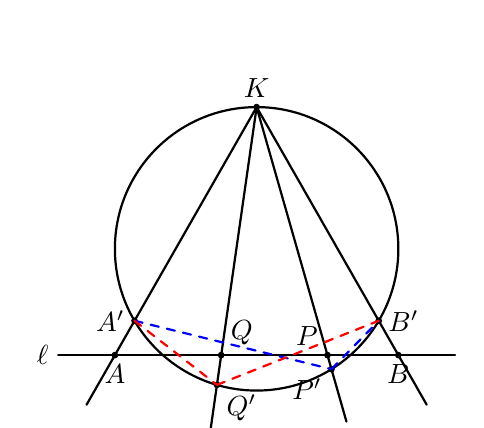
\begin{tikzpicture}[scale=0.9]
        \tkzDefPoints{-2/-.5/A, 2/-.5/B, 1/-.5/P, -0.5/-.5/Q, 0/1/O, 0/3/K}         
        \tkzInterLC[common = K](K,A)(O,K) \tkzGetFirstPoint{A'}
        \tkzInterLC[common = K](K,B)(O,K) \tkzGetFirstPoint{B'}
        \tkzInterLC[common = K](K,P)(O,K) \tkzGetFirstPoint{P'}
        \tkzInterLC[common = K](K,Q)(O,K) \tkzGetFirstPoint{Q'}
        \tkzDrawPoints[fill=black](A,B,P,Q,K,A',B',P',Q')
        \tkzDrawCircle[black, thick](O,K)
        \tkzDrawLines[black, thick](A,B)
        \tkzDrawLines[black, thick,add=0 and 0.2](K,A K,Q' K,P' K,B)
        \tkzLabelLine[left, pos=-0.2](A,B){$\ell$}
        \tkzDrawSegments[blue, thick, dashed](A',P' P',B')
        \tkzDrawSegments[red, thick, dashed](A',Q' Q',B')
        \tkzLabelPoints[above left](P)
        \tkzLabelPoints[above right](Q)
        \tkzLabelPoints[right](B')
        \tkzLabelPoints[left](A')
        \tkzLabelPoints[below](A,B)
        \tkzLabelPoints[below right](Q')
        \tkzLabelPoints[below left](P')
        \tkzLabelPoints[above](K)
    \end{tikzpicture}
    \label{fig:cr_lc}
    \caption{線-圓射影交比不變性}
\end{figure}
\end{mybox}
\begin{mybox}{4.5em}{1em}{0.5em}
證明與性質3的證明一致，讀者可以自行驗證其正確性。
\end{mybox}
\begin{mybox}[性質4的其他情況]{9.5em}{1em}{0.5em}
關於定理4，點列$\left(A,B,P,Q\right)$與點列$\left(A',B',P',Q'\right)$還有其他不同的分佈情況，任何一種情況都滿足線-圓射影不變性。
以下列舉四種不同的情況，讀者可以自行驗證其正確性。
\end{mybox}
\begin{figure}[H]
    \centering
    \begin{subfigure}[b]{0.4\textwidth}
        \centering
        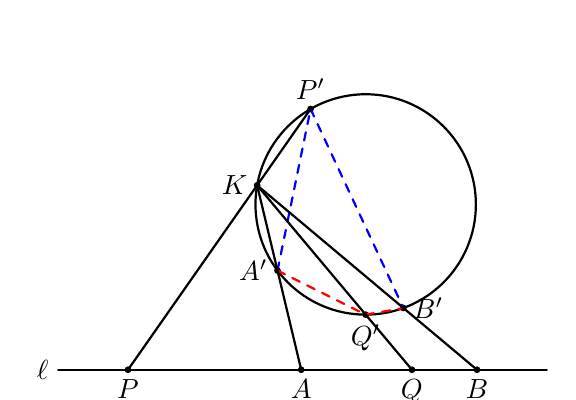
\begin{tikzpicture}[scale = 0.7]
            \tkzDefPoints{0/0/O, -2/0/A'',-1.6/-1.2/A', -2/-3/C, 2/-3/D}
            \tkzDefPointBy[rotation= center O angle -60](A'') \tkzGetPoint{P'}
            \tkzDefPointBy[rotation= center O angle 90](A'') \tkzGetPoint{Q'}
            \tkzDefPointBy[rotation= center O angle 110](A'') \tkzGetPoint{B'}
            \tkzDefPointBy[rotation= center O angle -10](A'') \tkzGetPoint{K}
            \tkzInterLL(K,A')(C,D) \tkzGetPoint{A}
            \tkzInterLL(K,B')(C,D) \tkzGetPoint{B}
            \tkzInterLL(K,P')(C,D) \tkzGetPoint{P}
            \tkzInterLL(K,Q')(C,D) \tkzGetPoint{Q}
            \tkzDrawPoints[black](A,B,P,Q,K,A',B',P',Q')
            \tkzDrawCircle[black, thick](O,K)
            \tkzDrawSegments[blue, thick, dashed](A',P' P',B')
            \tkzDrawSegments[red, thick, dashed](A',Q' Q',B')
            \tkzDrawSegments[black, thick](K,A K,B P,P' K,Q)
            \tkzDrawLine[black, thick, add=0.2 and 0.2](P,B)
            \tkzLabelLine[left, pos=-0.2](P,B){$\ell$}
            \tkzLabelPoints[left](A',K)
            \tkzLabelPoints[above](P')
            \tkzLabelPoints[right](B')
            \tkzLabelPoints[below](Q',A,B,P,Q)
        \end{tikzpicture}
    \end{subfigure}
    \hfill
    \begin{subfigure}[b]{0.4\textwidth}
        \centering
        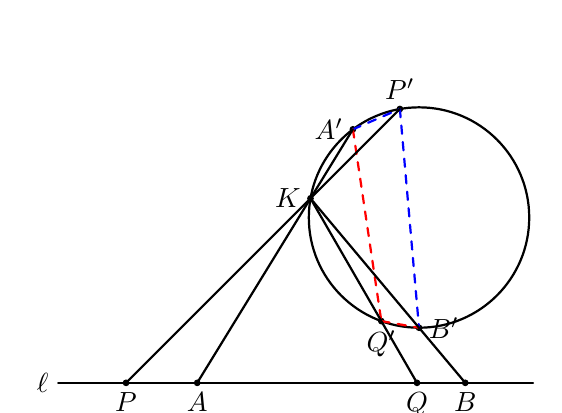
\begin{tikzpicture}[scale = 0.7]
            \tkzDefPoints{0/0/O, -2/0/A'',-1.2/1.6/A', -2/-3/C, 2/-3/D}
            \tkzDefPointBy[rotation= center O angle -80](A'') \tkzGetPoint{P'}
            \tkzDefPointBy[rotation= center O angle 70](A'') \tkzGetPoint{Q'}
            \tkzDefPointBy[rotation= center O angle 90](A'') \tkzGetPoint{B'}
            \tkzDefPointBy[rotation= center O angle -10](A'') \tkzGetPoint{K}
            \tkzInterLL(K,A')(C,D) \tkzGetPoint{A}
            \tkzInterLL(K,B')(C,D) \tkzGetPoint{B}
            \tkzInterLL(K,P')(C,D) \tkzGetPoint{P}
            \tkzInterLL(K,Q')(C,D) \tkzGetPoint{Q}
            \tkzDrawPoints[black](A,B,P,Q,K,A',B',P',Q')
            \tkzDrawCircle[black, thick](O,K)
            \tkzDrawSegments[blue, thick, dashed](A',P' P',B')
            \tkzDrawSegments[red, thick, dashed](A',Q' Q',B')
            \tkzDrawSegments[black, thick](A',A K,B P,P' K,Q)
            \tkzDrawLine[black, thick, add=0.2 and 0.2](P,B)
            \tkzLabelLine[left, pos=-0.2](P,B){$\ell$}
            \tkzLabelPoints[left](A',K)
            \tkzLabelPoints[above](P')
            \tkzLabelPoints[right](B')
            \tkzLabelPoints[below](Q',A,B,P,Q)
        \end{tikzpicture}
    \end{subfigure}
    \vspace{1em}
    \begin{subfigure}[b]{0.4\textwidth}
        \centering
        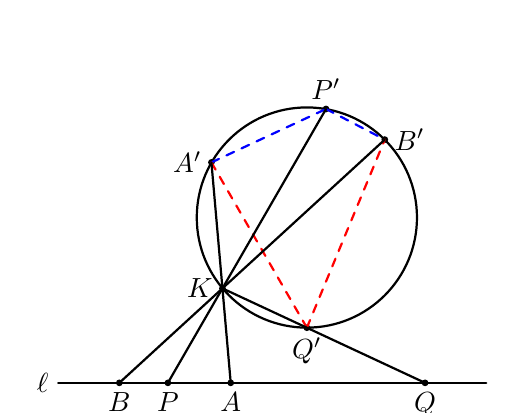
\begin{tikzpicture}[scale = 0.7]
            \tkzDefPoints{0/0/O, -2/0/A'', -2/-3/C, 2/-3/D}
            \tkzDefPointBy[rotation= center O angle -30](A'') \tkzGetPoint{A'}
            \tkzDefPointBy[rotation= center O angle -100](A'') \tkzGetPoint{P'}
            \tkzDefPointBy[rotation= center O angle 90](A'') \tkzGetPoint{Q'}
            \tkzDefPointBy[rotation= center O angle -135](A'') \tkzGetPoint{B'}
            \tkzDefPointBy[rotation= center O angle 40](A'') \tkzGetPoint{K}
            \tkzInterLL(K,A')(C,D) \tkzGetPoint{A}
            \tkzInterLL(K,B')(C,D) \tkzGetPoint{B}
            \tkzInterLL(K,P')(C,D) \tkzGetPoint{P}
            \tkzInterLL(K,Q')(C,D) \tkzGetPoint{Q}
            \tkzDrawPoints[black](A,B,P,Q,K,A',B',P',Q')
            \tkzDrawCircle[black, thick](O,K)
            \tkzDrawSegments[blue, thick, dashed](A',P' P',B')
            \tkzDrawSegments[red, thick, dashed](A',Q' Q',B')
            \tkzDrawSegments[black, thick](A',A B',B P,P' K,Q)
            \tkzDrawLine[black, thick, add=0.2 and 0.2](B,Q)
            \tkzLabelLine[left, pos=-0.2](B,Q){$\ell$}
            \tkzLabelPoints[left](A',K)
            \tkzLabelPoints[above](P')
            \tkzLabelPoints[right](B')
            \tkzLabelPoints[below](Q',A,B,P,Q)
        \end{tikzpicture}
    \end{subfigure}
    \hfill
    \begin{subfigure}[b]{0.4\textwidth}
        \centering
        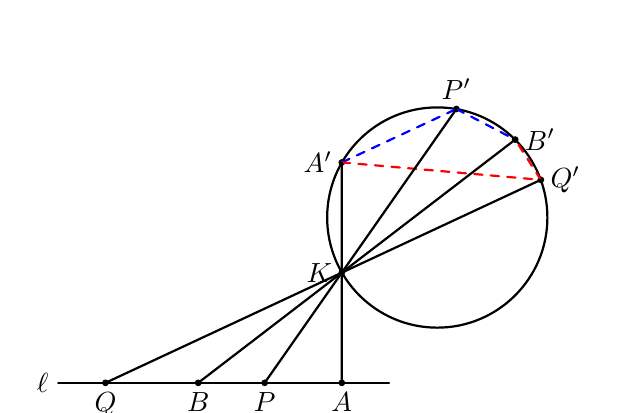
\begin{tikzpicture}[scale = 0.7]
            \tkzDefPoints{0/0/O, -2/0/A'', -2/-3/C, 2/-3/D}
            \tkzDefPointBy[rotation= center O angle -30](A'') \tkzGetPoint{A'}
            \tkzDefPointBy[rotation= center O angle -100](A'') \tkzGetPoint{P'}
            \tkzDefPointBy[rotation= center O angle -160](A'') \tkzGetPoint{Q'}
            \tkzDefPointBy[rotation= center O angle -135](A'') \tkzGetPoint{B'}
            \tkzDefPointBy[rotation= center O angle 30](A'') \tkzGetPoint{K}
            \tkzInterLL(K,A')(C,D) \tkzGetPoint{A}
            \tkzInterLL(K,B')(C,D) \tkzGetPoint{B}
            \tkzInterLL(K,P')(C,D) \tkzGetPoint{P}
            \tkzInterLL(K,Q')(C,D) \tkzGetPoint{Q}
            \tkzDrawPoints[black](A,B,P,Q,K,A',B',P',Q')
            \tkzDrawCircle[black, thick](O,K)
            \tkzDrawSegments[blue, thick, dashed](A',P' P',B')
            \tkzDrawSegments[red, thick, dashed](A',Q' Q',B')
            \tkzDrawSegments[black, thick](A',A B',B P,P' Q',Q)
            \tkzDrawLine[black, thick, add=0.2 and 0.2](Q,A)
            \tkzLabelLine[left, pos=-0.2](Q,A){$\ell$}
            \tkzLabelPoints[left](A',K)
            \tkzLabelPoints[above](P')
            \tkzLabelPoints[right](B',Q')
            \tkzLabelPoints[below](A,B,P,Q)
        \end{tikzpicture}
    \end{subfigure}
\end{figure}
\begin{mybox}[性質5]{4.5em}{1em}{0.5em}
    （性質4的極限情況）：在任意圓$\Gamma$上任取四個相異點$A'$、$B'$、$P'$、$Q'$，任取直線$\ell$，
    設$\ell$分別與直線$A'B'$、$A'P'$和$A'Q'$相交於$B$、$P$和$Q$三點，而過$A'$點的切線與直線$\ell$相交於$A$點，則有以下關係式成立：
    $$
        \left(A',B';P',Q'\right)=\left(A,B;P,Q\right)
    $$
    \begin{figure}[H]
        \centering
        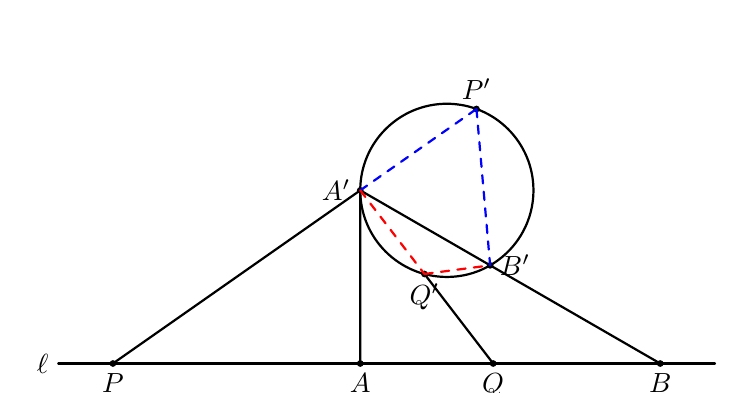
\begin{tikzpicture}[scale=1.1]
            \tkzDefPoints{0/0/O, -1/0/A', 0/-2/C, 1/-2/D, -1/1/E}
            \tkzDefPointBy[rotation= center O angle 120](A') \tkzGetPoint{B'}  
            \tkzDefPointBy[rotation=center O angle 75](A') \tkzGetPoint{Q'}
            \tkzDefPointBy[rotation=center O angle -110](A') \tkzGetPoint{P'}
            \tkzInterLL(A',B')(C,D) \tkzGetPoint{B}
            \tkzInterLL(A',P')(C,D) \tkzGetPoint{P}
            \tkzInterLL(A',Q')(C,D) \tkzGetPoint{Q}
            \tkzInterLL(E,A')(C,D) \tkzGetPoint{A}
            \tkzDrawPoints[fill=black](A,B,P,Q,A',B',P',Q')
            \tkzDrawCircle[black, thick](O,A')
            \tkzDrawLines[black, thick, add=0.1 and 0.1](P,B)
            \tkzLabelLine[left, pos=-0.1](P,B){$\ell$}
            \tkzDrawSegments[black, thick](A',A A',B A',P Q',Q)
            \tkzDrawSegments[blue, thick, dashed](A',P' P',B')
            \tkzDrawSegments[red, thick, dashed](A',Q' Q',B')
            \tkzLabelPoints[right](B')
            \tkzLabelPoints[left](A')
            \tkzLabelPoints[below](A,B,P,Q,Q')
            \tkzLabelPoints[above](P')
        \end{tikzpicture}
        \label{fig:cr_lc_limit}
        \caption{線-圓射影交比不變性（極限情況）}
    \end{figure}
\end{mybox}
\section{調和點列}
在介紹完有向交比和無向交比的定義及性質後，我們將引入一個非常重要的概念——調和點列。
這個概念亦是數學競賽中的幾何常見題型，時常配合着角平分線或調和四邊形一起出現。

介紹調和點列之前，首先要引入另一個概念——無窮遠點：
\begin{mybox}[無窮遠點]{6em}{1em}{0.5em}
    故名思義，無窮遠點是一個存在於無窮遠處的點。
    
    對於空間上任一條直線，「無窮遠點$\infty$」皆在直線上。

    在歐氏幾何中，一對平行線永不相交，但是在射影幾何中，一對平行線是會相交於「無窮遠點$\infty$」的。

    對於任意兩點$A$、$B$，無窮遠點$\infty$的有向分割比為
    $$
        \overrightarrow{A\infty}/\overrightarrow{\infty B}=-1
    $$
    上式可以視為無窮遠點的「數值定義」。
\end{mybox}
\begin{mybox}[調和點列（定義1）]{10.5em}{1em}{0.5em}
    對於同一直線上的四個相異點$A$、$B$、$P$和$Q$，如果$\left(A,B;P,Q\right)=-1$，則稱四點$A$、$B$、$P$和$Q$為一組\underline{調和點列}。
\end{mybox}
\begin{mybox}[調和點列（定義2）]{10.5em}{1em}{0.5em}
    對於同一直線上的四個相異點$A$、$B$、$P$和$Q$，如果$\left[A,B;P,Q\right]=1$，則稱四點$A$、$B$、$P$和$Q$為一組\underline{調和點列}。
\end{mybox}
\end{document}